\documentclass{article}
\usepackage[utf8]{inputenc}
\usepackage[T1]{fontenc}
\usepackage{tabto}
\usepackage{fancyvrb}
\usepackage{graphicx}
\usepackage{geometry}
\usepackage{listings}

\title{Laboratorium 1}
\author{Szymon Kałuża}
\date{08.03.2022}

\begin{document}
\newgeometry{lmargin=0.5cm, rmargin=0.5cm, tmargin=0.5cm, bmargin=0.5cm}
\maketitle
\section{Zadanie 1}
\subsection{a)}
Dla zbioru danych wejściowych data.txt:\\
\VerbatimInput{data2.txt}
\endgroup
Przy pomocy gnu plot dokonano aproksymacji funkcji $an^2+bn+c$
\\\\
\#Key means label...\\
set title "Zaleznosc czasu dzialania algorytmu od jego zlozonosci"\\
set style data linespoints\\
set style line 1 lt 1 lw 6\\
set pointsize 1.5\\
set ylabel 'Czas pracy T(n) w sekundach'\\
set xlabel 'Rozmiar danych wejsciowych'\\
set tics nomirror out\\
set style line 101 lc rgb '\#000000' lt 1 lw 1\\
set border 3 front ls 101\\
set style line 102 lc rgb '\#d6d7d9' lt 0 lw 1\\
set grid back ls 102\\
set format x '%g'\\
\\
fit a*x**2+b*x+c "data.dat" via a,b,c;\\
plot "data.dat" using 1:2 title 'Dane doswiadczalne' with lines, $a*x**2+b*x+c$ t '$f(x)=n^2$'\\
Otrzymano następujące wyniki:\\
\VerbatimInput{test1.txt}
\endgroup
\begin{figure}[bhp]
    \centering
    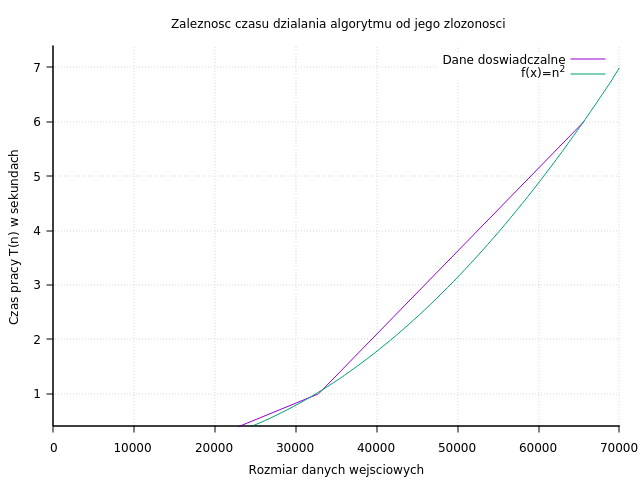
\includegraphics[width=4in,height=3in]{zadanie1.png}
    \caption{Zależność czasu działania algorytmu do rozmiaru danych }
    \label{fig:my_label}
\end{figure}
\subsection{b)}
Program:\\
Nieniejszy program jest podstawą dla całego zadania 1!
\begin{lstlisting}
void selectSort(int* tab, int noe)
{
    for(int i = 0; i <= noe -2; i++)
    {
        int min = i;
        for(int j = i + 1; j <= noe -1; )
        {
            if(tab[j] < tab[min])
            {
                min = j;
            }
            j++;
        }
        change(tab, i, min);
    }
}

void change(int* tab, int i, int min)
{
    int temp = tab[i];
    tab[i] = tab[min];
    tab[min] = temp;
}
\end{lstlisting}
Hipoteza:\\
Czas działania naszego programu spełnia prawo potęgowe:
$T(N) = a \cdot N^b dla b = 3$, tj.\\ $$T(N)= a \cdot N^2$$
Obliczenia:\\
Wartość stałej a:
a = $0,114219/8192^2 = 0,00000000170199573040008544921875\\
przewidywanie:\\
$T(n) = 0,00000000170199573040008544921875 \cdot 16384^2 = 0,456876$\\
$T(N) = 0,00000000170199573040008544921875 \cdot 32768^2 = 1,827504$\\
$T(N) = 0,00000000170199573040008544921875 \cdot 65536^2 = 7,310016$\\
\begin{table}[bhp]
    \begin{tabular}{|c|c|c|c|c|}
    \hline
        il. el & czas & wsp. zmiany & logN & czas/$il el^2$\\ \hline
    	128.0 & 3.7E-5 &  & \  & \  \\ \hline
    	256.0 & 1.46E-4 & 3.945945946 & 1.980371193 & 0.000000002227783203 \\ \hline
    	512.0 & 7.03E-4 & 4.815068493 & 2.26755632 & 0.000000002681732178 \\ \hline
    	1024.0 & 0.001977 & 2.812233286 & 1.491716277 & 0.000000001885414124 \\ \hline
    	2048.0 & 0.007053 & 3.567526555 & 1.834924169 & 0.000000001681566238 \\ \hline
    	4096.0 & 0.027985 & 3.967815114 & 1.988344803 & 0.000000001668035984 \\ \hline
    	8192.0 & 0.114219 & 4.081436484 & 2.029077006 & 0.00000000170199573 \\ \hline
    	16384.0 & 0.4654 & 4.074628564 & 2.026668552 & 0.000000001733750105 \\ \hline
    	32768.0 & 1.826972 & 3.925595187 & 1.972911408 & 0.000000001701500267 \\ \hline
    	65536.0 & 6.7084 & 3.671867987 & 1.876514191 & 0.00000000156192109 \\ \hline
    \end{tabular}
    \caption{Select sort zależność czasu do ilości danych}
    \label{tab:my_label}
\end{table}
\\Jak widać na przedstawionej powyżej tabeli nasza hipoteza została potwierdzona, dane otrzymane z obliczeń są porównywalne z danymi wynikającymi z przeprowadzonych testów.
\section{Zadanie 2}
\subsection{a)}
Dla zbioru danych wejściowych data2.txt:\\
\VerbatimInput{data2.txt}
Przy pomocy gnu plot dokonano aproksymacji funkcji $an^2+bn+c$
\\\\
\#Key means label...\\
set title "Zaleznosc czasu dzialania algorytmu od jego zlozonosci"\\
set style data linespoints\\
set style line 1 lt 1 lw 6\\
set pointsize 1.5\\
set ylabel 'Czas pracy T(n) w sekundach'\\
set xlabel 'Rozmiar danych wejsciowych'\\
set tics nomirror out\\
set style line 101 lc rgb '\#000000' lt 1 lw 1\\
set border 3 front ls 101\\
set style line 102 lc rgb '\#d6d7d9' lt 0 lw 1\\
set grid back ls 102\\
set format x '%g'\\
\\
\\
fit a*x**2+b*x+c "data.dat" via a,b,c;\\
plot "data.dat" using 1:2 title 'Dane doswiadczalne' with lines, $a*x**2+b*x+c$ t 'f(x)=n^2'\\
\\
\endgroup
Otrzymano następujące wyniki:\\
\VerbatimInput{test2.txt}
\begin{figure}[bhp]
    \centering
    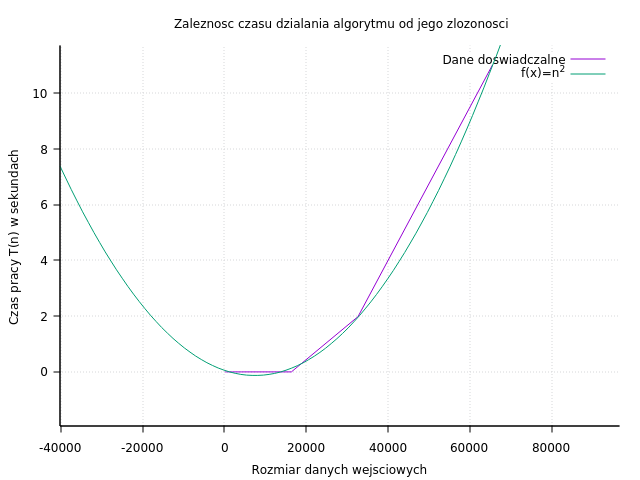
\includegraphics[width=4in,height=3in]{zadanie2.png}
    \caption{Zależność czasu działania algorytmu do rozmiaru danych}
    \label{fig:my_label}
\end{figure}
\subsection{b)}
Program:
Nieniejszy program jest podstawą dla całego zadania 2 !
\begin{lstlisting}
void change(int* tab, int i, int min)
{
    int temp = tab[i];
    tab[i] = tab[min];
    tab[min] = temp;
}

void bubbleSort(int* tab, int noe)
{
    for(int i = 0; i < noe - 1; i++)
    {
        for(int j = i; j < noe - 1; j++)
        {
            if(tab[j] < tab[j-1])
            {
                change(tab, j, j-1);
            }
        }
    }
}
\end{lstlisting}
Hipoteza:\\
Czas działania naszego programu spełnia prawo potęgowe: $T(N) = a \cdot N^b$ dla b = 2, tj. $$T(N) = a \cdot N^2$$

obliczenia:\\
Wartość stałej a: $a =  0.139693/8192^2 = 2,08158791065216064453125e-9$\\
Przewidywania:\\
$T(N) = 2,08158791065216064453125e-9 \cdot 16384^2=0,558772$\\
$T(N) = 2,08158791065216064453125e-9 \cdot 32768^2=2,235088$\\
$T(N) = 2,08158791065216064453125e-9 \cdot 65536^2=8,940352$\\
\begin{table}[bhp]
    \centering
    \begin{tabular}{|c|c|c|c|c|}
        \hline
        il. el & czas & wsp. zmiany & logN & czas/$il el^2$\\ \hline
    	128.0 & 3.9E-5 & \  & \  & \  \\ \hline
    	256.0 & 1.43E-4 & 3.666666667 & 1.874469118 & 0.000000002182006836 \\ \hline
    	512.0 & 6.3E-4 & 4.405594406 & 2.139336682 & 0.000000002403259277 \\ \hline
    	1024.0 & 0.002195 & 3.484126984 & 1.800797206 & 0.000000002093315125 \\ \hline
    	2048.0 & 0.008681 & 3.954897494 & 1.983640302 & 0.000000002069711685 \\ \hline
    	4096.0 & 0.034284 & 3.949314595 & 1.981602295 & 0.000000002043485641 \\ \hline
    	8192.0 & 0.139693 & 4.074582896 & 2.026652382 & 0.000000002081587911 \\ \hline
    	16384.0 & 0.605784 & 4.33653798 & 2.116543745 & 0.000000002256721258 \\ \hline
    	32768.0 & 2.737241 & 4.518509898 & 2.175847083 & 0.000000002549254335 \\ \hline
    	65536.0 & 11.461985 & 4.187422664 & 2.066062546 & 0.000000002668701345 \\ \hline

    \end{tabular}
    \caption{Caption}
    \label{tab:my_label}
\end{table}\\
Jak widać na przedstawionej powyżej tabeli, dane pochodzące z obliczeń zawyżają czas działania programu, jednak oscylują około prawidłowych wartości. Można więc uznać, że nasza hipoteza została potwierdzona.
\end{document}